\documentclass[a4paper, 14pt]{extarticle}
\usepackage[utf8]{inputenc}
\usepackage[paper=a4paper, top=1cm, right=1cm, bottom=1.5cm, left=2cm]{geometry}
\usepackage{setspace}
\onehalfspacing

\usepackage{graphicx}
\graphicspath{{plots/}, {images/}}

\parindent=1.25cm

\usepackage{titlesec}

\titleformat{\section}
    {\normalsize\bfseries}
    {\thesection}
    {1em}{}

\titleformat{\subsection}
    {\normalsize\bfseries}
    {\thesubsection}
    {1em}{}

% Настройка вертикальных и горизонтальных отступов
\titlespacing*{\chapter}{0pt}{-30pt}{8pt}
\titlespacing*{\section}{\parindent}{*4}{*4}
\titlespacing*{\subsection}{\parindent}{*4}{*4}

\usepackage[square, numbers, sort&compress]{natbib}
\makeatletter
\bibliographystyle{unsrt}
\renewcommand{\@biblabel}[1]{#1.} 
\makeatother


\newcommand{\maketitlepage}[6]{
    \begin{titlepage}
        \singlespacing
        \newpage
        \begin{center}
            Министерство образования и науки Российской Федерации \\
            Федеральное государственное бюджетное образовательное \\
            учреждение высшего профессионального образования \\
            <<Волгоградский государственный технический университет>> \\
            #1 \\
            Кафедра #2
        \end{center}


        \vspace{14em}

        \begin{center}
            \large Семестровая работа #6 по дисциплине
            \\ <<#3>>
        \end{center}

        \vspace{5em}

        \begin{flushright}
            \begin{minipage}{.35\textwidth}
                Выполнила:\\#4
                \vspace{1em}\\
                Проверил:\\#5
                \\
                \\ Оценка \underline{\ \ \ \ \ \ \ \ \ \ \ \ \ \ \ \ }
            \end{minipage}
        \end{flushright}

        \vspace{\fill}

        \begin{center}
            Волгоград, \the\year
        \end{center}

    \end{titlepage}
    \setcounter{page}{2}
}

\newcommand{\maketitlepagewithvariant}[7]{
    \begin{titlepage}
        \singlespacing
        \newpage

        \begin{center}
            Министерство образования и науки Российской Федерации \\
            Федеральное государственное бюджетное образовательное \\
            учреждение высшего профессионального образования \\
            <<Волгоградский государственный технический университет>> \\
            #1 \\
            Кафедра #2
        \end{center}


        \vspace{8em}

        \begin{center}
            \large Семестровая работа #6 по дисциплине
            \\ <<#3>>
        \end{center}

        \vspace{1em}
        \begin{center}
            Вариант №#7
        \end{center}
        \vspace{4em}

        \begin{flushright}
            \begin{minipage}{.35\textwidth}
                Выполнила:\\#4
                \vspace{1em}\\
                Проверил:\\#5
                \\
                \\ Оценка \underline{\ \ \ \ \ \ \ \ \ \ \ \ \ \ \ \ }
            \end{minipage}
        \end{flushright}

        \vspace{\fill}

        \begin{center}
            Волгоград, \the\year
        \end{center}

    \end{titlepage}
    \setcounter{page}{2}
}

\input{../../../.preambles/10-russian}
\input{../../../.preambles/20-math}
\input{../../../.preambles/22-vectors}
\input{../../../.preambles/30-physics}
\usepackage{mathrsfs}

\renewcommand{\labelenumi}{\asbuk{enumi})}
\newcommand{\ds}{\displaystyle}
\newcommand{\inv}{\mathrm{inv}}
\renewcommand{\v}{\mathrm{v}}
\newcommand{\E}{\mathscr{E}}

\begin{document}
\maketitlepage{Факультет электроники и вычислительной техники}{физики}
{Электродинамика}{2}{}{студентка группы Ф-369\\Слоква~В.~И.}{f}
{доцент Грецов~М.~В.}{m}

\newpage
% ------------------------------------------------------------------------------
\emph{705.} Длинный прямой цилиндрический катод радиуса \( a \), по которому
течет равномерно распределенный ток \( I \), испускает электроны с нулевой
начальной скоростью. Эти электроны движутся под действием ускоряющего
потенциала \( V \) к длинному коаксиальному аноду радиуса \( b \). Каково
должно быть минимальное значение разности потенциалов \( V_\emph{кр} \) между
катодом и анодом, чтобы электроны достигали анода, несмотря на заворачивающее
действие магнитного поля тока \( I \)?

\vspace*{2em}
\emph{Решение:}

\begin{minipage}{.4\textwidth}
    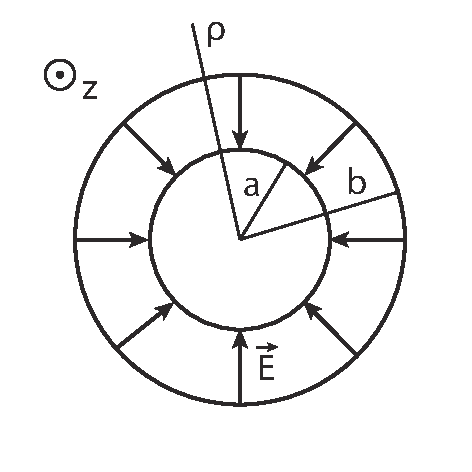
\includegraphics[width=\textwidth]{2-1}
\end{minipage}
\begin{minipage}{.55\textwidth}
Проекции уравнения движения
\[
    \der{p}{t} = e\vec{E} + e\vec{v}\times\vec{B}
\]
на оси \( \rho \) и \( z \):
\begin{gather*}
    \der{p_\rho}{t} = eE; \\
    \der{p_z}{t} = ev_\rho B,
\end{gather*}
так как \( \vec{v}\perp\vec{B} \) и \( \vec{v}\times\vec{B} = v_\rho B\vec{e}_z
\).
\end{minipage}

Полная энергия электрона в поле:
\[
    \E = c\sqrt{p^2 + m^2c^2} + \frac{\alpha}{r},
\]
где \( \alpha = ee' \), \( e' = -e \):
\[
    mc^2 = \sqrt{p^2c^2 + m^2c^4} - eV.
\]

Выражаем \( eV \):
\[
    eV = \sqrt{(cp)^2 + m^2c^4} - mc^2.
\]

\( p = p_z \), так как нас интересует крайний случай, при котором еще
наблюдается долет электрона до анода. Тогда:
\begin{gather*}
    dp_z = ev_\rho B\,dt; \\
    dp_z = eB\d\rho; \\
    \int\limits_0^{p_z} dp_z = e\int\limits_a^b B\d\rho.
\end{gather*}

По закону Био-Савара:
\[
    B = \frac{\mu\mu_0 J}{2\pi\rho}.
\]

Перейдя для удобства в СГС, получаем:
\[
    B = \frac{4\pi}{c^2}\frac{J}{2\pi\rho} = \frac{2J}{c^2\rho}.
\]

Тогда \( p_z \):
\[
    p_z = e\int\limits_a^b \frac{2J}{c^2}\frac{d\rho}{\rho} = \frac{2Je}{c^2}
    \ln\frac{b}{a}.
\]

А \( eV_\emph{кр} \) тогда:
\begin{gather*}
    eV_\emph{кр} = \sqrt{\frac{4J^2e^2}{c^2}\ln^2\frac{b}{a} + m^2c^4} - mc^2 =
    mc^2\sqrt{\frac{e^2}{m^2c^4}\cdot\frac{4J^2}{c^2}\ln^2\frac{b}{a} + 1} -
    mc^2 \approx \\
    \approx mc^2\left(1 + \frac{e^2}{m^2c^4}\cdot\frac{2J^2}{c^2}\ln^2
    \frac{b}{a}\right) - mc^2 = \frac{e^2}{mc^2}\cdot\frac{2J^2}{c^2}\ln^2
    \frac{b}{a},
\end{gather*}

откуда
\[
    V_\emph{кр} = \frac{2J^2e}{mc^4}\ln^2\frac{b}{a}.
\]
\vspace*{2em}
\emph{Ответ:} \( V_\emph{кр} = \cfrac{2J^2e}{mc^4}\ln^2\cfrac{b}{a} \).
    
\newpage

%-------------------------------------------------------------------------------
\emph{749.} Центры двух электрических дипольных осцилляторов с частотой
\( \omega \) и одинаковой амплитудой \( p_0 \| x \) находятся на оси \( z \), на
равных расстояниях от начала координат и на расстоянии \( a = \lambda/4 \) друг
от друга. Колебания в осцилляторах сдвинуты по фазе на \( \pi/2 \). Найти
угловое распределение излучения \( \ds \mid{\der{I}{\Omega}} \).

\vspace*{2em}
\emph{Решение:}

\begin{minipage}{.4\textwidth}
    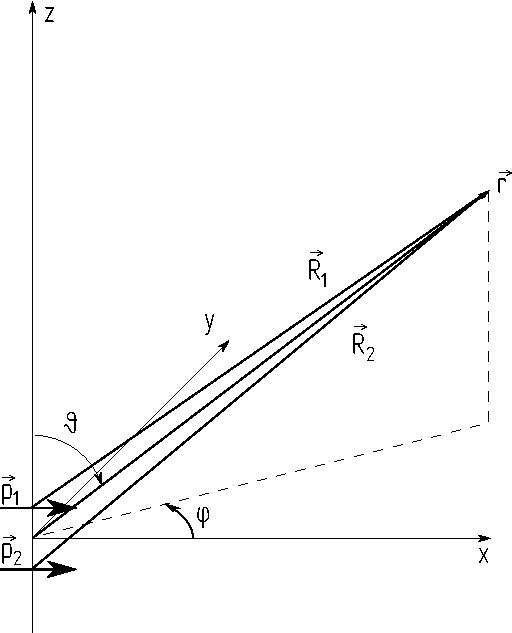
\includegraphics[width=\textwidth]{2-2}
\end{minipage}
\begin{minipage}{.55\textwidth}
Для удобства рассмотрения будем решать задачу в сферических координатах.
\[
    \frac{dW}{dt\,d\Omega} = |\vec{P}|\cdot r^2,
\]
где \( \vec{P} \) -- вектор Пойнтинга. Считая в волновой зоне участок фронта
волны вблизи точки наблюдения плоским, можем записать, что
\[
    P = \frac{c}{\mu_0}B^2.
\]

Считая волну монохроматической и усредняя по времени, имеем
\end{minipage}
\[
    \der{I}{\Omega} = \frac{cr^2}{2\mu_0}B_0^2,
\]
где \( B_0 \) -- амплитудное значение индукции магнитного поля в
рассматриваемой точке.

Индукция магнитного поля, создаваемого в точке волновой зоны дипольным
осциллятором может быть записана в виде
\[
    \vec{B} = \frac{\mu_0\omega^2\vec{p}_{t-\frac{R}{c}}\times\vec{n}}{4\pi Rc}.
\]

Для двух близко расположенных диполей получаем
\[
    \vec{B} = \vec{B}_1 + \vec{B}_2 =
    \frac{\mu_0\omega^2\vec{p}_{t-\frac{R_1}{c}}\times\vec{n_1}}{4\pi R_1c} +
    \frac{\mu_0\omega^2\vec{p}_{t-\frac{R_2}{c}+\frac{T}{4}}\times\vec{n_2}}
    {4\pi R_2c}.
\]
Не сделав большой ошибки, можем принять в знаменателях \( R_1 = R_2 = r \), а в
числителях \( R_1 = r - \frac{1}{2}{a\cos\theta},\ R_2 = r + \frac{1}{2}
{a\cos\theta} \) и \( \vec{n_1} = \vec{n_2} = \vec{n} \). Тогда получаем
выражение
\[
    \vec{B} = \frac{\mu_0\omega^2(p_{t-\frac{r}{c}+
    \frac{1}{2}{\frac{a}{c}\cos\theta}}+p_{t-\frac{r}{c}-
    \frac{1}{2}{\frac{a}{c}\cos\theta}+\frac{T}{4}})\vec{e}_x\times\vec{n}}
    {4\pi rc}.
\]
Рассмотрим сумму дипольных моментов, стоящую в скобках. Перейдём к комплексам:
\begin{align*}
    & \hat{p}_{t-\frac{r}{c}+\frac{1}{2}{\frac{a}{c}\cos\theta}} +
    \hat{p}_{t-\frac{r}{c}-\frac{1}{2}{\frac{a}{c}\cos\theta}+\frac{T}{4}} =
    p_0(e^{i\omega(t-\frac{r}{c}+\frac{1}{2}{\frac{a}{c}\cos\theta)}} +
    e^{i\omega(t-\frac{r}{c}-\frac{1}{2}{\frac{a}{c}\cos\theta}+\frac{T}{4})})=
    \\ &=
    p_0e^{i\omega(t-\frac{r}{c})}(e^{i\omega\frac{1}{2}\frac{a}{c}\cos\theta} +
    e^{i\omega(-\frac{1}{2}{\frac{a}{c}\cos\theta}+\frac{T}{4})}) = 
    p_0e^{i\omega(t-\frac{r}{c})}e^{i\frac{\pi}{4}}\sqrt{2}
    \cos\left(\frac{a\omega}{2c}\cos{\theta} + \frac{\pi}{4}\right) =\\
    &=
    p_0\sqrt{2}\cos\left(\frac{\pi}{2}\cos^2\frac{\theta}{2}\right)
    e^{i\omega(t-\frac{r}{c})}e^{i\frac{\pi}{4}}.
\end{align*}
Заметим также, что
\[
    |\vec{e}_x\times\vec{n}| = \sqrt{1-\sin^2\theta\cos^2\phi}
\]
Для амплитуды магнитного поля получаем выражение
\[
    B_0 = \frac{\mu_0\omega^2p_0\sqrt{2}
    \cos\left(\frac{\pi}{2}\cos^2\frac{\theta}{2}\right)
    \sqrt{1-\sin^2\theta\cos^2\phi}}{4\pi rc}.
\]
Подставляя в выражение для интенсивности, в конечном итоге имеем
\[
    \der{I}{\Omega} = \frac{\mu_0\omega^4p_0^2}{16\pi^2 c}
    (1-\sin^2\theta\cos^2\phi)
    \cos^2\left(\frac{\pi}{2}\cos^2\frac{\theta}{2}\right).
\]

\emph{Ответ:} \( \ds
    \der{I}{\Omega} = \frac{\mu_0\omega^4p_0^2}{16\pi^2 c}
    (1-\sin^2\theta\cos^2\phi)
    \cos^2\left(\frac{\pi}{2}\cos^2\frac{\theta}{2}\right).
\)

\newpage

%-------------------------------------------------------------------------------
\emph{770.} Релятивистская частица с зарядом \( e \), массой \( m \) и импульсом
\( p \) движется по круговой орбите в постоянном однородном магнитном поле
\( \vec{H} \). Радиус орбиты \( a = cp/eH \). Найти суммарную по всем
направлениям скорость потери энергии частицей \( \ds \left(-\der{\E}
{t'}\right) \).

\vspace*{2em}
\emph{Решение:}
Уравнение движения частицы в магнитном поле \( \vec{H} \):
\[
    \der{\vec{p}}{t'} = \frac{e}{c}\vec{v}\times\vec{H}.
\]

Изменение скорости:
\[
    \der{\vec{v}}{t'} = \vec{v}\times\frac{e\vec{H}}{mc} = \frac{\vec{p}}{m}
    \times\frac{p\vec{e}_H}{ma} = \frac{p^2}{am^2}\vec{e}_p\times\vec{e}_H =
    \frac{v^2}{a}\vec{e}_p\times\vec{e}_H.
\]

\begin{minipage}{.4\textwidth}
    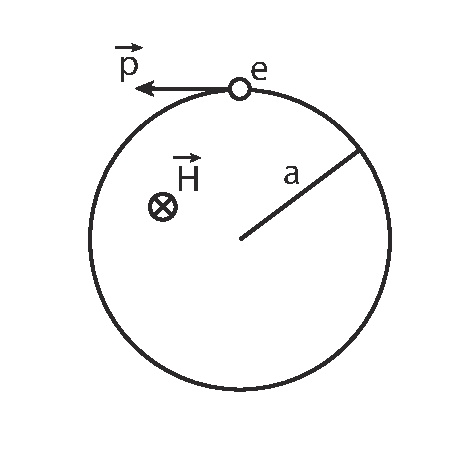
\includegraphics[width=\textwidth]{2-3}
\end{minipage}
\begin{minipage}{.55\textwidth}
В результате излучения ускоренно движущаяся частица теряет энергию и импульс,
передавая их электромагнитному полю. Потерю \( i \)-й составляющей 4-вектора
энергии--импульса \( p_i = \left( \cfrac{\E}{c},\ \vec{p} \right) \) в единицу
собственного времени \( \tau \) можно выразить через 4-скорость \( u_i \) и
4-ускорение \( w_i \) частицы:
\[
    -\der{p_i}{\tau} = \frac{2e^2}{3c^3} w_k^2 u_i.
\]
\end{minipage}

Потеря энергии:
\[
    -\frac{1}{c}\der{\E}{\tau} = \frac{2e^2}{3c^3} w_k^2 u_0^2.
\]

В лабораторной системе отсчета скорость потери энергии отличается множителем
\( \gamma = \cfrac{1}{\sqrt{1-v^2/c^2}} \), так как \( dt' = \gamma\d\tau \):
\[
    -\gamma\der{\E}{t'} = \frac{2e^2}{3c^2} w_k^2 u_0.
\]

Так как временная компонента 4-скорости совпадает с \( c\gamma \),то
\[
    -\der{\E}{t'} = \frac{2e^2}{3c} w_k^2.
\]

Так как частица движется по окружности, то поле \( \vec{H} \) перпендикулярно
импульсу \( \vec{H} \perp \vec{p} \), а ее ускорение \( w = \cfrac{v^2}{a} =
w_k \). Его квадрат:
\[
    w^2 = \left(\frac{v^2}{a}\right)^2 = \left(\frac{p^2eH}{m^2cp}\right)^2 =
    \frac{p^2e^2H^2}{m^4c^2}.
\]

Тогда потеря энергии:
\[
    -\der{\E}{t'} = \frac{2p^2e^4H^2}{3m^4c^5}.
\]

\vspace*{2em}
\emph{Ответ:} \( \ds -\der{\E}{t'} = \frac{2p^2e^4H^2}{3m^4c^5} \).
\end{document}
